\documentclass[a4paper,11pt]{article}
\usepackage{wisebed-tr}
\usepackage{longtable}
\usepackage{placeins}
\urlstyle{same}



\newenvironment{apidoc}[6]%
{%

		\begin{longtable}[t]{p{2cm}p{12.8cm}}
      Semantics	 & #2 \\[0.5em]
	    Signature	 & \lstinline{#1}\\[0.5em]
	    Parameters & {#3} \\[0.5em]
      Returns		 & #4 \\[0.5em]
      Rationale \tabularnewline for changes & #5 \\[0.5em]
      Since 		 & #6 \\[0.5em]
		\end{longtable}

 	
%	}
	\begingroup
%  }%
%  {
  \endgroup
}	


\newcommand{\apiparameters}[1]	{\hspace{-0.25cm}\begin{tabular}[t]{lp{10cm}} #1 \end{tabular}}

\newcommand{\apiparam}[2]	{ \lstinline{#1} & #2 \\ }
	

	\delivNumber{TR-RS-API-V1}
	\delivTitle{Reservation System API (RS API)}
	\delivAuthor{UZL, UBERN, ULANC}
	\delivDate{\today}

%---------------------------------------------------------
%  	Document Start 
%---------------------------------------------------------

\begin{document}
    \prepareTitle

%---------------------------------------------------------------------------
	\section{Introduction}
	\label{sec:introduction}
%---------------------------------------------------------------------------
This document describes the Reservation System API (RS API). This API is part of a larger family of APIs which are defined by the WISEBED consortium for reserving, accessing, managing, and using a testbed. The RS API is responsible for reserving (parts of) a (potentially federated) testbed. All APIs are specified as standard Web Services using WSDL documents and a human-readable documentation. The Web Services comply to the WS-Interoperability Basic Profile~\cite{wsi-basic-profile-1-1}. All these APIs are ``federatable'' (cf. Section~\ref{sec:federatability}). At present, the following APIs exist:

\begin{itemize}
	\item Sensor Network Authentication and Authorization (SNAA API)
	\item Reservation System (RS API)
	\item Wireless Sensor Network API (WSN API) including its Sub-APIs:
	\begin{itemize}
		\item Session Management API
		\item Controller API
	\end{itemize}
\end{itemize}

Concerning implementations of this API, WISEBED already provides a set to choose from. For further information and download links, please refer to \url{http://www.wisebed.eu}. The remainder of this document is structured as follows. Section~\ref{sec:concepts} introduces standard concepts used throughout WISEBED, Section~\ref{sec:operations} describes the individual Web Service Operations, and Section~\ref{sec:appendix} contains the WSDL description and XML Schema document containing the data types.

%---------------------------------------------------------------------------
	\section{Concepts}
	\label{sec:concepts}
%---------------------------------------------------------------------------

%---------------------------------------------------------------------------
	\subsection{Node addressing}
	\label{sec:addressing}
%---------------------------------------------------------------------------
WISEBED uses Uniform Resource Names (URNs) to identify sensor nodes, node capabilities, edge attributes, node attributes, testbed portal servers, and points of interest. For more details, we refer the reader to WISEBED Deliverable D2.2 (Report on the Implementation of the Software Infrastructure) on \url{http://www.wisebed.eu}.

We define \textit{sensor nodes }as the unique nodes comprising each of the testbeds. Each sensor node belongs to only one \textit{sensor network}. A partner \textit{site} can be comprised of a number of such sensor networks. So, each sensor node of the federation is described using the unique ID of the partner site, a sensor network ID which is unique in the partner site namespace, and the sensor node ID which is unique in the specific sensor network scope it belongs to. 

\begin{lstlisting}
<URN> ::= ``urn:wisebed:node:<site>:<node id>''
\end{lstlisting}\medskip

\noindent Example: 

\begin{lstlisting}
urn:wisebed:node:cti:gw1:n1
urn:wisebed:node:cti:gw1:n8
urn:wisebed:node:uzl:building64:n33
urn:wisebed:node:ulanc:n876
\end{lstlisting}\medskip

A number of nodes share a common \emph{URN prefix}, e.g. urn:wisebed:node:cti or urn:wisebed:node:ulanc.

%---------------------------------------------------------------------------
	\subsection{Federatability}
	\label{sec:federatability}
%---------------------------------------------------------------------------
From a user's perspective, it must not matter whether he uses a local, small-scale testbed or a worldwide federation of testbeds -- or even a simulated testbed. This requires an architecture where a single testbed has the same interface towards the user as a federation of testbeds. It is therefore imperative that all interfaces, data formats, and interaction patterns are exactly the same -- independent of the type of the testbed. The goal is to come up with a generalized architecture that, amongst others, can be used 

\begin{itemize}
	\item to integrate additional testbeds in the federation, 
	\item to run private testbeds using the same APIs and their implementations,
	\item that allows third parties to operate their own testbeds (from desktop-size to a full-blown experimental facility), and 
	\item that supports the integration of simulated nodes into the experiment. 
\end{itemize}

An important aspect is that the APIs (and therefore also their implementations) are ``federatable''. Figure~\ref{fig:federation} further illustrates this concept. Here, a number of testbeds comprised of heterogeneous wireless sensor nodes are shown (a simplified WISEBED federation, a third-party testbed, and a simulated testbed using Shawn). 

 \begin{figure*}[htb]
      \begin{center}
      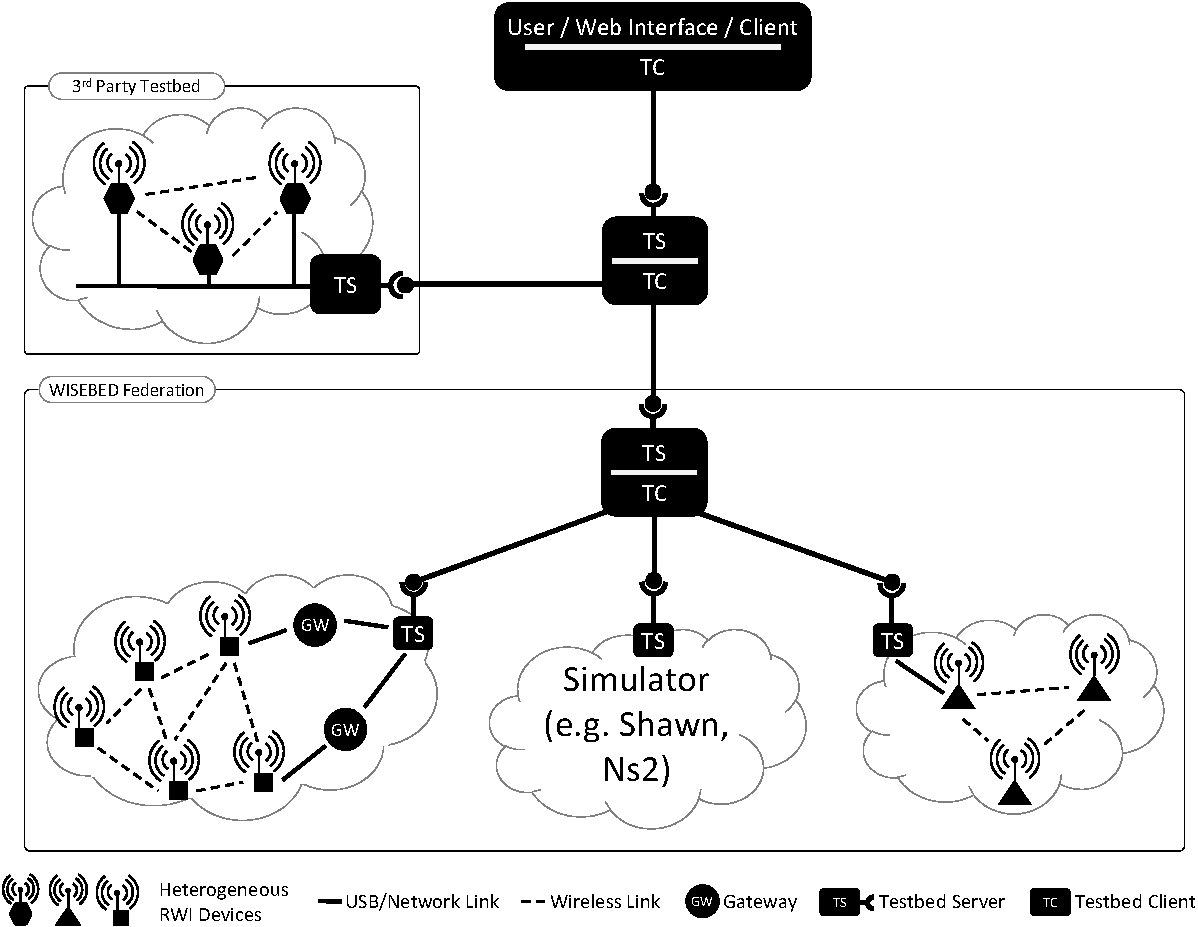
\includegraphics[width=.9\textwidth]{fig/federation}
      \caption{Federation hierarchy}
      \label{fig:federation}
      \end{center}
\end{figure*}

Each testbed (with or without a wired backbone or simulated) exposes its features using Web Services to the Internet (labeled Testbed Server, TS). Each client (Testbed Client, TC) uses these APIs to access the testbed (including AAA, reservation, reprogramming of nodes, sending messages to/receiving messages from nodes, etc.). A special client-side implementation, a so-called \emph{federator}, connects to several Testbed Servers and again exposes a Testbed Client to the Internet. Like this, multiple testbeds are federated and their features are exposed using as a single Testbed Server instance. As shown in Figure~\ref{fig:federation}, WISEBED uses this technology for exposing its distributed testbeds as a single experimental facility. This federation can then again be used to create an even larger federation using the same approach and so on. For a client, a federated testbed looks exactly like a single, non-distributed testbed. 

\FloatBarrier

%---------------------------------------------------------------------------
	\sectionfin
	\section{Operations}
	\label{sec:operations}
%---------------------------------------------------------------------------

%---------------------------------------------------------------------------
			\sectionfin
			\subsection{Make Reservation}
%---------------------------------------------------------------------------
	
\begin{apidoc}
	{List<SecretReservationKey> makeReservation(List<SecretAuthenticationKey> authenticationData, ConfidentialReservationData reservation) throws AuthorizationExceptionException, RSExceptionException, ReservationConflictExceptionException;} %Signature
	{Reserves a set of nodes for an interval of time} % Semantics
	{
			\apiparameters{
				\apiparam{authenticationData}{A sequence of $(urnprefix, secretauthenticationkey)$ tuples. These were obtained from a call to authorize() using the SNAA API.}
				\apiparam{reservation}{Which nodes to reserve for which time interval.}
			}
	} % Parameters
	{A $(urnprefix, secretreservationkey)$ tuple for corresponding input tuple or a fault otherwise} % Returns
	{} % Rationale for addition/changes
	{1.0} % Since
\end{apidoc}

This function is used to reserve a set of nodes for a certain time interval. 

The first parameter contains the secret authentication keys that were returned by a call to authorize() of the SNAA. The reservation system then invokes isAuthorized() with these keys and a (yet to be defined) string for the action parameter to determine whether a user is authorized to perform this reservation. 

The second parameter contains a list of node URNs that are to be reserved from $from$ until $to$ (inclusive). The parameter $userData$ can include arbitrary (public) information about the reservation. This could be used to store additional information about this reservation used by the client to the RS.

In addition, the RS must check whether the reservation can be made, i.e. if all the requested nodes are available for the requested time interval. 

If authorization and feasibility is given for ALL the nodes, it returns a set of $(urnprefix, secretreservationkey)$ tuples for each corresponding input tuple or a fault otherwise. If the reservation is not feasible due to conflicts with other reservations, a ReservationConflict fault is signaled. For other RS-internal faults, a RS fault is returned.

The request and response messages of this function are visualized in Figure~\ref{fig:make-reservation-request} and \ref{fig:make-reservation-response}.
	
	\myfig[\textwidth]{make-reservation-request}{Make reservation request}
	\myfig[\textwidth]{make-reservation-response}{Make reservation response}

%---------------------------------------------------------------------------
			\sectionfin
			\subsection{Delete Reservation}
%---------------------------------------------------------------------------

\begin{apidoc}
	{public void deleteReservation(List<SecretReservationKey> secretReservationKey) throws RSExceptionException, ReservationNotFoundExceptionException;} %Signature
	{} % Semantics
	{
			\apiparameters{
				\apiparam{secretReservationKey}{A $(urnprefix, secretreservationkey)$ tuple identifying a single reservation as returned by makeReservation().}
			}
	} % Parameters
	{Nothing} % Returns
	{} % Rationale for addition/changes
	{1.0} % Since
\end{apidoc}

This function deletes a single reservation. If the reservation was not found, a ReservationNotFound fault is returned.  For other RS-internal faults, a RS fault is returned. The request and response messages of this function are visualized in Figure~\ref{fig:delete-reservation-request} and \ref{fig:delete-reservation-response}.

	\myfig[\textwidth]{delete-reservation-request}{Delete reservation request}
	\myfig[\textwidth]{delete-reservation-response}{Delete reservation response}
		
%---------------------------------------------------------------------------
			\sectionfin
			\subsection{Get Reservations}
%---------------------------------------------------------------------------

\begin{apidoc}
	{public List<PublicReservationData> getReservations(DateTime from, DateTime to) throws RSExceptionException;} %Signature
	{Returns reservations for a time interval (excluding confidential information).} % Semantics
	{
			\apiparameters{
				\apiparam{from}{Start time to search for reservations (inclusive)}
				\apiparam{to}{End time to search for reservations (inclusive)}
			}
	} % Parameters
	{A list of reservations not including confidential data.} % Returns
	{} % Rationale for addition/changes
	{1.0} % Since
\end{apidoc}

This functions returs non-confidential reservation data for a certain time interval. The structure of the request is shown in Figure~\ref{fig:get-reservations-request}. This is useful for users to find out which nodes are available at which time before calling makeReservation. It could also be used to display a calendar. The structure of the response is shown in Figure~\ref{fig:get-reservations-response}. It is a list of reservations and contains information about which nodes are reserved for which intervals. 

	\myfig[\textwidth]{get-reservations-request}{}
	\myfig[\textwidth]{get-reservations-response}{}
	
%---------------------------------------------------------------------------
			\sectionfin
			\subsection{Get Reservation}
%---------------------------------------------------------------------------
	
\begin{apidoc}
	{public List<ConfidentialReservationData> getReservation(List<SecretReservationKey> secretReservationKey) throws RSExceptionException, ReservationNotFoundExceptionException;} %Signature
	{Returns data about a single reservation (including confidential information)} % Semantics
	{
			\apiparameters{
				\apiparam{secretReservationKey}{A $(urnprefix, secretreservationkey)$ tuple identifying a single reservation as returned by makeReservation().}
			}
	} % Parameters
	{Information about a certain reservation.} % Returns
	{} % Rationale for addition/changes
	{1.0} % Since
\end{apidoc}
	
This function returns details about a certain reservation. The parameter is shown in Figure~\ref{fig:get-reservation-request}. The returned data is shown in Figure~\ref{fig:get-reservation-response} which resembles the arguments to makeReservation(). If the reservation was not found, a ReservationNotFound fault is returned.  For other RS-internal faults, a RS fault is returned. 

Please note that this function returns confidential data such as the username. This is fine since the secretReservationKey is only known to the RS, the user and later the Session Management API. 

	\myfig[\textwidth]{get-reservation-request}{Request to getReservation}
	\myfig[\textwidth]{get-reservation-response}{Response of getReservation}

%---------------------------------------------------------------------------
			\sectionfin
			\subsection{Get Confidential Reservations}
%---------------------------------------------------------------------------

\begin{apidoc}
	{public List<ConfidentialReservationData> getConfidentialReservations(List<SecretAuthenticationKey> secretAuthenticationKey, GetReservations period) throws RSExceptionException;} %Signature
	{Returns reservations for a time interval (including confidential information)} % Semantics
	{
			\apiparameters{
				\apiparam{secretAuthenticationKey}{A $(urnprefix, secretreservationkey)$ tuple identifying a single reservation as returned by makeReservation().}
					\apiparam{period}{The period of time for which to return the data (from and to inclusive).}
			}
	} % Parameters
	{} % Returns
	{Required by user interfaces of the RS.} % Rationale for addition/changes
	{1.1} % Since
\end{apidoc}

	\myfig[\textwidth]{get-confidential-reservations-request}{}
	\myfig[\textwidth]{get-confidential-reservations-response}{}
	
	
%---------------------------------------------------------------------------
			\sectionfin
			\subsection{Faults}
%---------------------------------------------------------------------------
	
	\myfig[.5\textwidth]{reservation-conflict-fault}{}
	\myfig[.5\textwidth]{reservation-not-found-fault}{}
	\myfig[.5\textwidth]{authorization-fault}{}
	\myfig[.5\textwidth]{rs-fault}{}

    
    
%--------------------------------------------------------------------------------------------------------
	\sectionfin
	\section{Appendix}
	\label{sec:appendix}		
%--------------------------------------------------------------------------------------------------------
    
%---------------------------------------------------------------------------
			\subsection{WSDL}
%---------------------------------------------------------------------------

    	\lstinputlisting[language=WSDL,tabsize=1,basicstyle=\scriptsize]{../../wsdl/RS.wsdl}

%---------------------------------------------------------------------------
			\subsection{Data Types (XML Schema)}
%---------------------------------------------------------------------------

    	\lstinputlisting[language=XMLSchema,tabsize=1,basicstyle=\scriptsize]{../../wsdl/RSTypes.xsd}

%--------------------------------------------------------------------------------------------------------
%--  References
%--------------------------------------------------------------------------------------------------------
	\sectionfin
	\addcontentsline{toc}{section}{References}
	\bibliographystyle{abbrv}
	\bibliography{references}

	\label{lastpage}
\end{document}
